
\section{intro}%
\label{sec:intro}

Contexte : ca peut être développer : cf les travaux antérieurs du groupe (10lignes par items)

\section{Amélioration des solutions PMF par ajout de traceurs spécifiques}%
\label{sec:amélioration_des_solutions_pmf}

\subsection{Isotopie}%
\label{sub:isotopie}

\subsection{Émission biogénique primaire}%
\label{sub:émission_biogénique_primaire}

\subsection{Processus secondaires}%
\label{sub:processus_secondaires}

\section{Confrontation des solutions PMF}%
\label{sec:confrontation_des_solutions_pmf}

\subsection{Autres modèles pour validation}%
\label{sub:autres_modèles_pour_validation}

14C, PSCF

\subsection{Incertitudes associées}%
\label{sub:incertitudes_associées}

\subsection{Comparabilité des solutions}%
\label{sub:comparabilité_des_solutions}

\section{SOURCES}%
\label{sec:sources}

\subsection{Introduction}

\subsection{Comparison of PM\textsubscript{10} Sources Profiles at 15 French Sites Using a Harmonized Constrained Positive Matrix Factorization Approach}%
\label{sub:article}

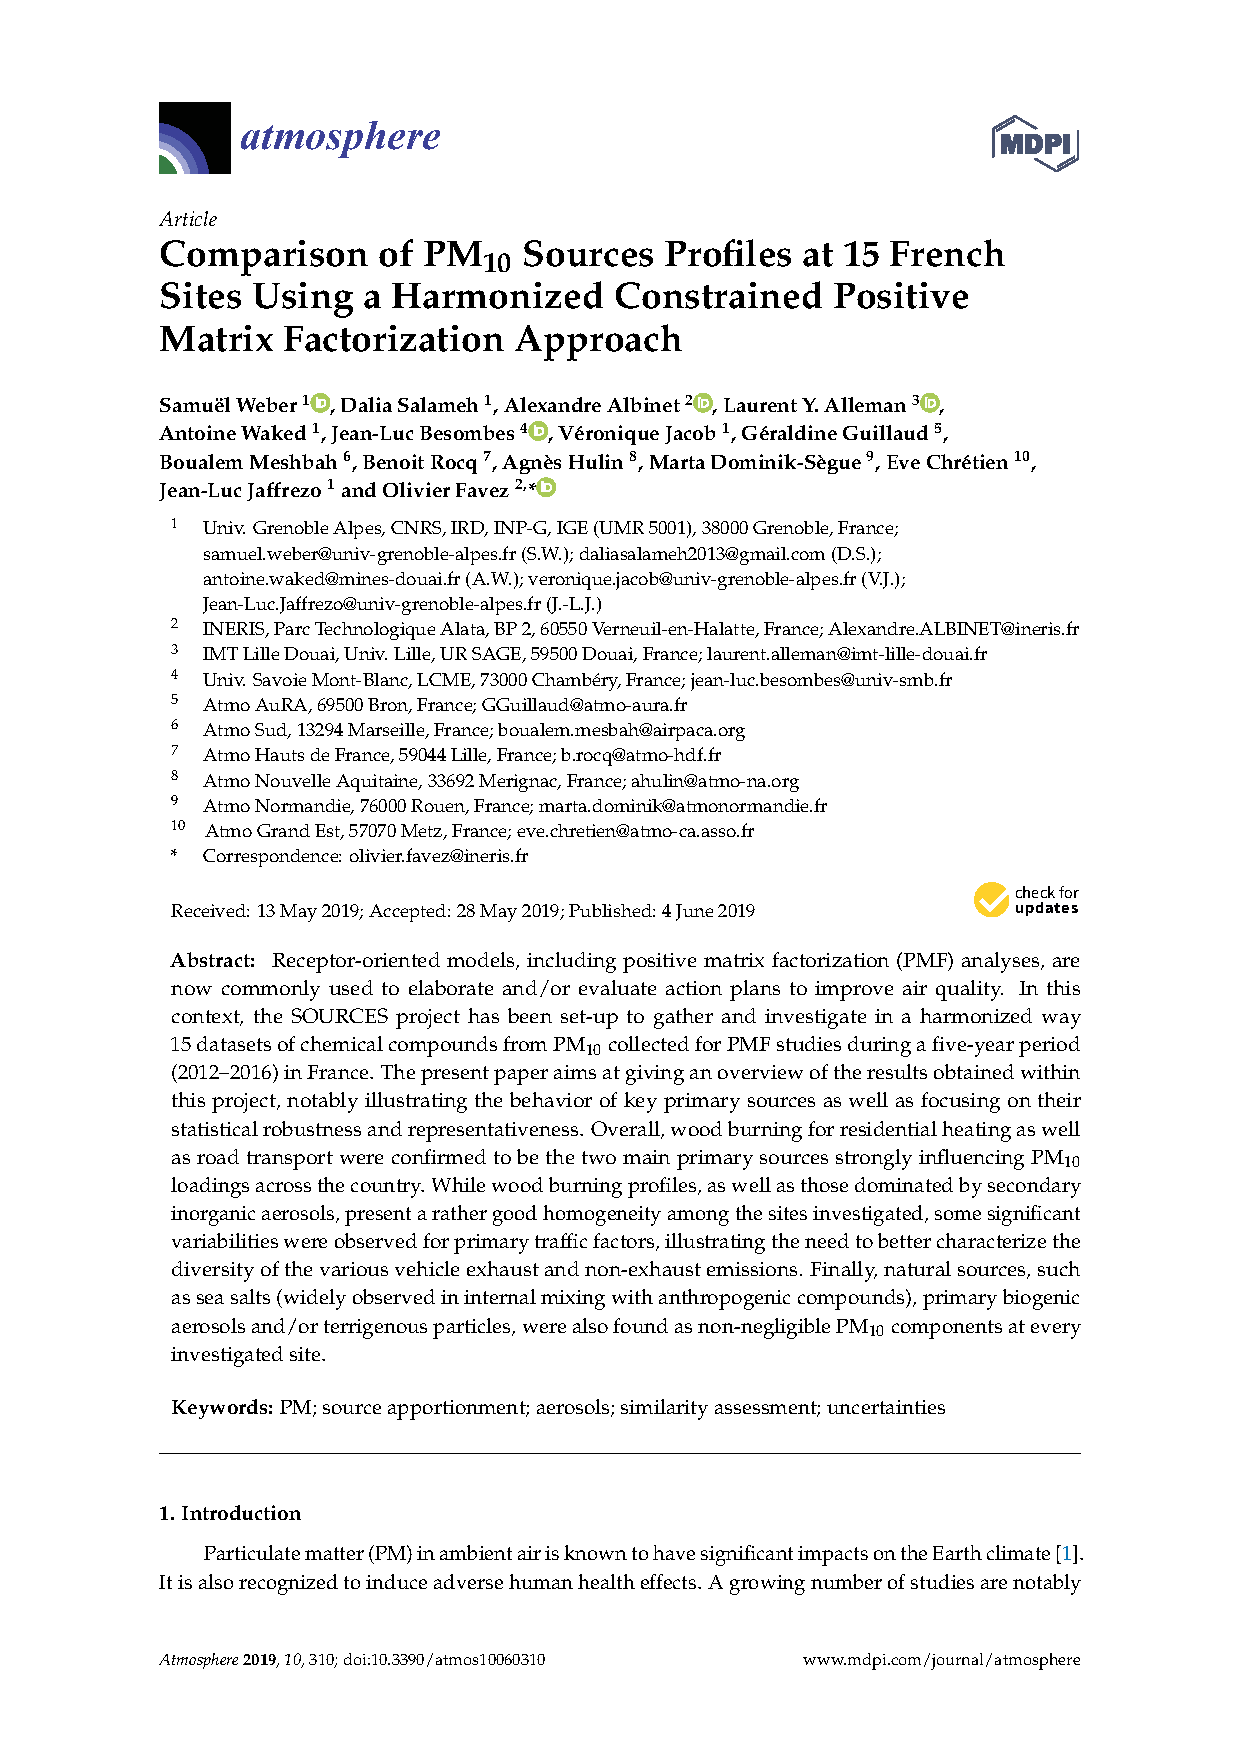
\includepdf[pages=-,scale=0.9,pagecommand={\pagestyle{fancy}}]{chapters/SOURCES.pdf}

\subsection{Supporting information}%
\label{sub:supporting_information}

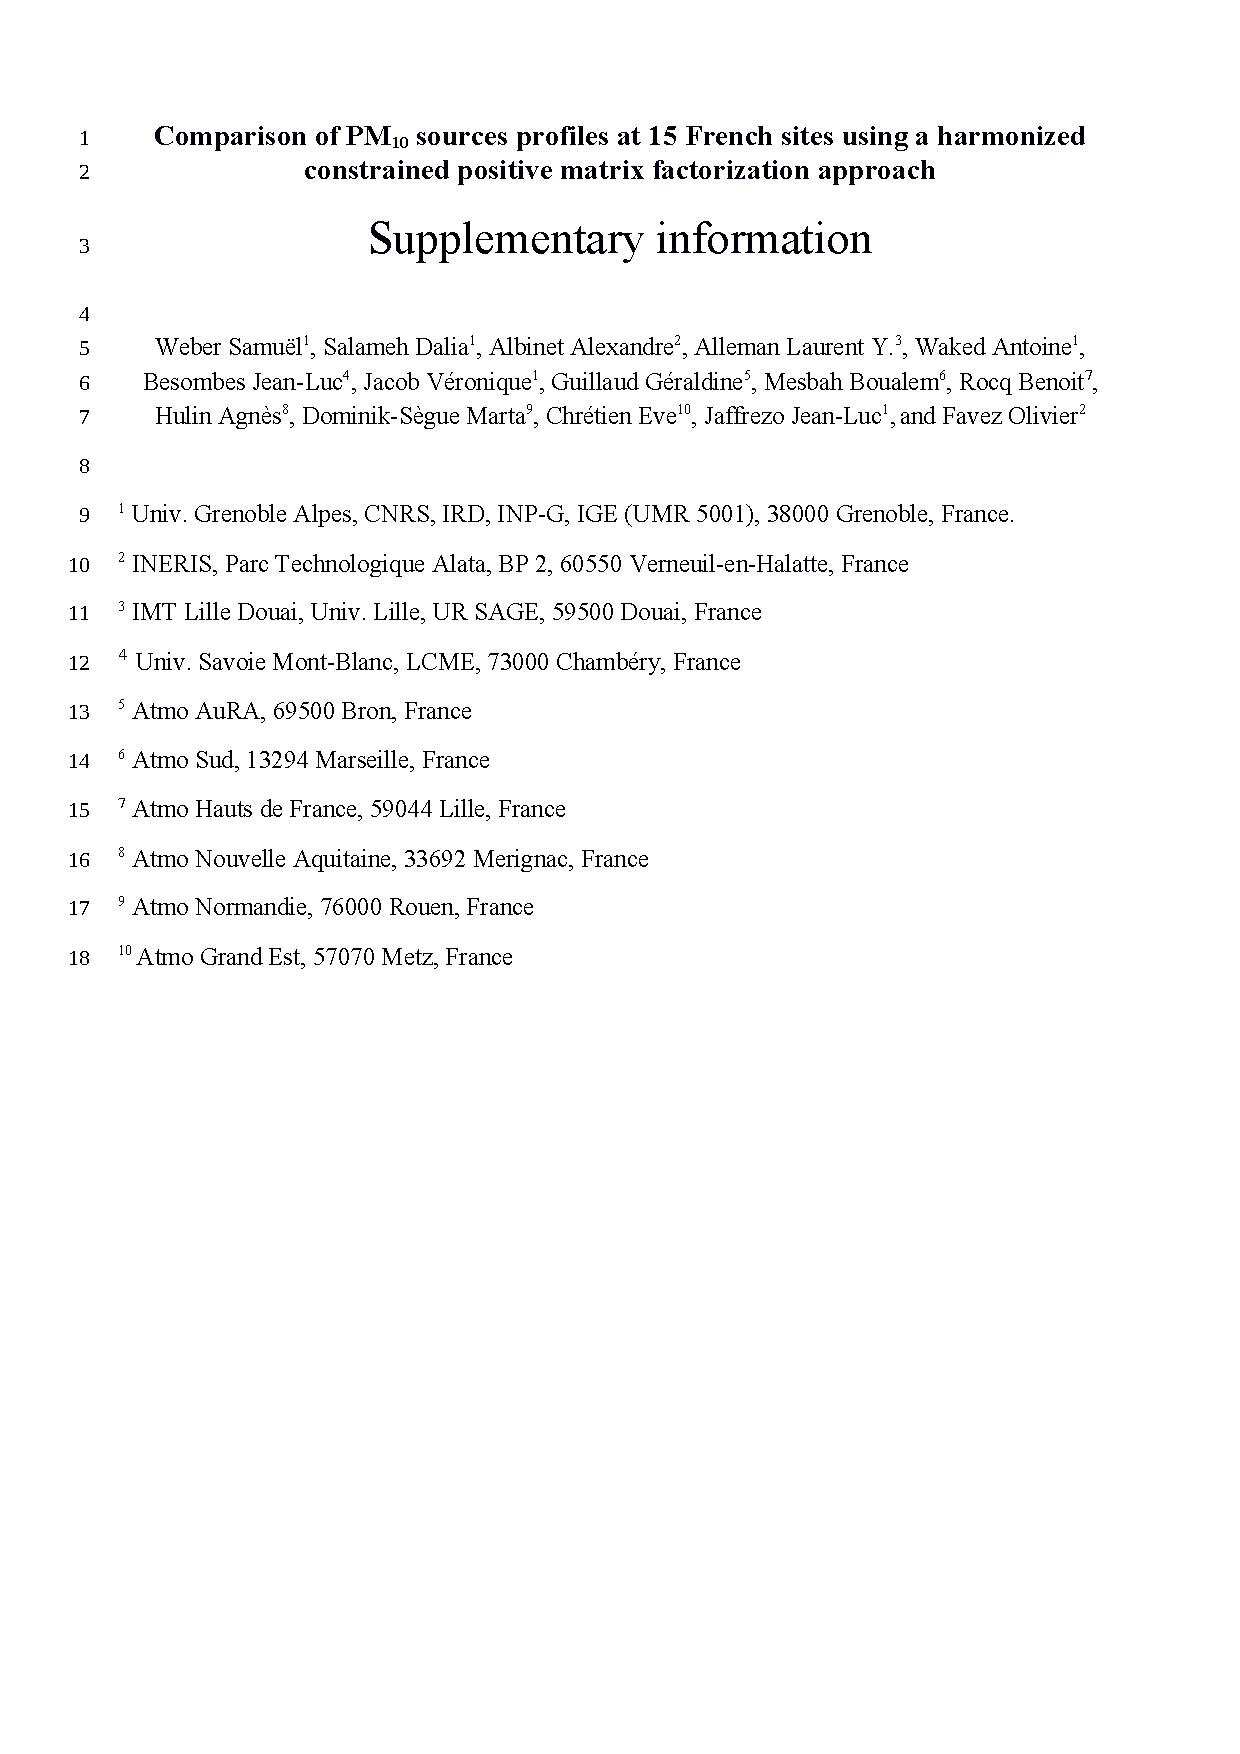
\includepdf[pages=-,scale=0.9,pagecommand={\pagestyle{fancy}}]{chapters/SOURCES_SI.pdf}


\section{conclusion}%
\label{sec:conclusion}

Et aussi LCME: organique (BNT, hopane), EMPA cellulose PM10/PM2.5

Question : SPECIEUROPE et contrainte trop fortes sur certains profils ?

Ouverture : ANDRA et série temporelle

Limitation : 
- espèce trop réactive ? (oxalate ?)
- résolution temporelle



